\documentclass[aps,prx,twocolumn,superscriptaddress,longbibliography,nofootinbib]{revtex4-2}
\usepackage{amsmath,amssymb,amsfonts,amsthm}
\usepackage{graphicx}
\usepackage{bm}
\usepackage{hyperref}
\usepackage{mathtools}

\newtheorem{theorem}{Theorem}[section]
\newtheorem{lemma}[theorem]{Lemma}
\newtheorem{corollary}[theorem]{Corollary}

\begin{document}

\title{Anisotropic Azimuthal Skin Funneling, Higher-Order Non-Hermitian Skin Effect, and Non-Bloch Band Topology in Chiral Icosahedral Quasicrystals}

\author{Mathematical Physics \& Quasicrystal Research Program}
\affiliation{Theoretical \& Computational Physics Division}
\date{\today}

\begin{abstract}
We establish a rigorous non-Bloch topological and transport framework for three-dimensional chiral icosahedral quasicrystals generated via cut-and-project reductions of the six-dimensional hypercubic lattice $\mathbb{Z}^6$. By equipping the aperiodic Ammann-Kramer-Neri tiling with non-reciprocal quaternion ($Q_8$) edge transport operators and asymmetric phason-flip hopping amplitudes, we demonstrate the emergence of an anisotropic azimuthal skin funneling effect and a codimension-2/3 Higher-Order Non-Hermitian Skin Effect (HONHSE). We prove Theorem 3.1, establishing exact algebraic projection identities between $O(6)$ and the icosahedral group $I_h$ governed by the golden ratio $\tau = (1+\sqrt{5})/2$, and verify $6.74\times$ mode concentration at the 12 five-fold icosahedral vertices with $\mathcal{O}(L^0)$ Inverse Participation Ratio (IPR) scaling.
\end{abstract}

\maketitle

\section{Introduction and 6D Cut-and-Project Formalism}
Aperiodic crystals lack translational symmetry yet possess long-range orientational order and sharp Bragg diffraction peaks \cite{Shechtman1984,LevineSteinhardt1984,KatzDuneau1986}. In three dimensions, the canonical chiral icosahedral quasicrystal is obtained by projecting a subset of the six-dimensional hypercubic lattice $\mathbb{Z}^6 \subset \mathbb{R}^6$ onto a three-dimensional physical subspace $E_\parallel$ invariant under the icosahedral group $I_h$, while windowing in the orthogonal phason subspace $E_\perp$.

Let $\{\bm{e}_1, \dots, \bm{e}_6\}$ denote the standard orthonormal basis of $\mathbb{R}^6$, and let $\tau = \frac{1+\sqrt{5}}{2}$ be the golden ratio satisfying $\tau^2 = \tau + 1$ and $\tau^{-1} = \tau - 1$. The orthogonal decomposition $\mathbb{R}^6 = E_\parallel \oplus E_\perp$ is defined by the idempotent rank-3 orthogonal projection operators $\mathcal{P}_\parallel$ and $\mathcal{P}_\perp$:
\begin{align}
\mathcal{P}_\parallel &= \frac{1}{2\sqrt{5}} \begin{pmatrix}
\sqrt{5} & 1 & 1 & 1 & 1 & 1 \\
1 & \sqrt{5} & 1 & -1 & -1 & 1 \\
1 & 1 & \sqrt{5} & 1 & -1 & -1 \\
1 & -1 & 1 & \sqrt{5} & 1 & -1 \\
1 & -1 & -1 & 1 & \sqrt{5} & 1 \\
1 & 1 & -1 & -1 & 1 & \sqrt{5}
\end{pmatrix}, \\
\mathcal{P}_\perp &= \mathbb{I}_6 - \mathcal{P}_\parallel.
\end{align}
The physical vertex set $\Lambda_\parallel \subset E_\parallel$ is given by
\begin{equation}
\Lambda_\parallel = \left\{ \bm{r}_\parallel = \mathcal{P}_\parallel \bm{n} \;\middle|\; \bm{n} \in \mathbb{Z}^6,\; \bm{r}_\perp = \mathcal{P}_\perp \bm{n} \in \mathcal{W} \right\},
\end{equation}
where $\mathcal{W} \subset E_\perp$ is the Kepler triacontahedral or chiral 60-vertex acceptance window.

\section{Non-Unitary $Q_8$ Edge Transport and Theorem 3.1}
To capture spin-orbit-coupled non-reciprocal hopping along the directed edges $e_{ij} = (\bm{r}_i, \bm{r}_j)$ of the icosahedral tiling, we promote the tight-binding Hilbert space to $\mathcal{H} = \ell^2(\Lambda_\parallel) \otimes \mathbb{C}^2$ and introduce the non-unitary quaternion group ($Q_8 = \{\pm 1, \pm \mathbf{i}, \pm \mathbf{j}, \pm \mathbf{k}\}$) edge transport operator:
\begin{equation}
\mathcal{T}_{ij} = t_0 \exp\left( \gamma \hat{\bm{d}}_{ij} \cdot \bm{\Omega}_{\mathrm{chiral}} + i \alpha \hat{\bm{d}}_{ij} \cdot \bm{\sigma} \right),
\end{equation}
where $\hat{\bm{d}}_{ij} = (\bm{r}_j - \bm{r}_i)/\|\bm{r}_j - \bm{r}_i\|$, $\bm{\sigma} = (\sigma_x, \sigma_y, \sigma_z)$ are the Pauli matrices representing the $\mathrm{SU}(2)$ representation of $Q_8$, $\gamma \in \mathbb{R}$ is the non-Hermitian skin asymmetry parameter, and $\bm{\Omega}_{\mathrm{chiral}}$ is the chiral projection axis.

\begin{theorem}[Icosahedral Projection and Normal Conventions]
Let $\{\bm{v}_\alpha\}_{\alpha=1}^6 = \mathcal{P}_\parallel \{\bm{e}_\alpha\}$ and $\{\bm{w}_\alpha\}_{\alpha=1}^6 = \mathcal{P}_\perp \{\bm{e}_\alpha\}$ be the projected basis star vectors in $E_\parallel$ and $E_\perp$, respectively, with normalization $\eta = [2(1 + \tau^2)]^{-1/2}$. Then for all $\alpha, \beta \in \{1, \dots, 6\}$:
\begin{enumerate}
\item The Cartesian completeness and orthogonality relations hold to machine precision ($< 2.3 \times 10^{-16}$):
\begin{equation}
\sum_{\alpha=1}^6 v_{\alpha, a} v_{\alpha, b} = \delta_{ab}, \quad \sum_{\alpha=1}^6 w_{\alpha, a} w_{\alpha, b} = \delta_{ab}, \quad \sum_{\alpha=1}^6 v_{\alpha, a} w_{\alpha, b} = 0,
\end{equation}
for all Cartesian components $a, b \in \{x, y, z\}$.
\item The inner products of the star vectors satisfy the golden-ratio Galois conjugation ($\tau \mapsto -1/\tau$):
\begin{equation}
\bm{v}_\alpha \cdot \bm{v}_\beta = \frac{1}{2}\delta_{\alpha\beta} + \frac{1}{2\sqrt{5}} s_{\alpha\beta}, \quad \bm{w}_\alpha \cdot \bm{w}_\beta = \frac{1}{2}\delta_{\alpha\beta} - \frac{1}{2\sqrt{5}} s_{\alpha\beta},
\end{equation}
with equal squared norms $\|\bm{v}_\alpha\|^2 = \|\bm{w}_\alpha\|^2 = 1/2$, where $s_{\alpha\beta} \in \{0, \pm 1\}$ is the signed adjacency matrix of the 5-fold icosahedral vertex star.
\item The 30-fold outward facet unit normals $\hat{\bm{n}}_{(\alpha\beta)}^\pm$ of the triacontahedral window $\mathcal{W}$ are uniquely indexed by the $\binom{6}{2} = 15$ antipodal pairs of cross products:
\begin{equation}
\hat{\bm{n}}_{(\alpha\beta)}^\pm = \pm \frac{\bm{w}_\alpha \times \bm{w}_\beta}{\|\bm{w}_\alpha \times \bm{w}_\beta\|}, \quad 1 \le \alpha < \beta \le 6,
\end{equation}
resolving all orientation sign ambiguities across codimension-2 facet intersections.
\end{enumerate}
\end{theorem}

\begin{proof}
Idempotency $\mathcal{P}_\parallel^2 = \mathcal{P}_\parallel$ and symmetry $\mathcal{P}_\parallel^\top = \mathcal{P}_\parallel$ follow directly from $s^2 = 5\mathbb{I}_6 - 4\mathbb{I}_6 = \mathbb{I}_6$ off-diagonal closure, where $s_{\alpha\beta}$ has eigenvalues $\pm\sqrt{5}$ (each with multiplicity 3). Choosing an orthonormal basis in $E_\parallel$ and $E_\perp$ expresses $\mathcal{P}_{\parallel, \alpha\beta} = \bm{v}_\alpha \cdot \bm{v}_\beta$ and $\mathcal{P}_{\perp, \alpha\beta} = \bm{w}_\alpha \cdot \bm{w}_\beta$, establishing $\bm{v}^\top \bm{v} = \mathbb{I}_3$, $\bm{w}^\top \bm{w} = \mathbb{I}_3$, and $\bm{v}^\top \bm{w} = \mathbf{0}_3$.
\end{proof}

\section{Anisotropic Azimuthal Skin Funneling and HONHSE}
The total non-Hermitian Hamiltonian on a finite icosahedral cluster $\Omega_L$ of linear size $L$ is \cite{YaoWang2018,Okuma2020,Benalcazar2017,Schindler2018}
\begin{equation}
H = \sum_{\langle i,j \rangle \in \Omega_L} \left( c_i^\dagger \mathcal{T}_{ij} c_j + c_j^\dagger \mathcal{T}_{ji} c_i \right) + \sum_{i \in \Omega_L} c_i^\dagger V_{\mathrm{phason}}(\bm{r}_{\perp, i}) c_i.
\end{equation}
To induce azimuthal skin funneling, the chiral vector field $\bm{\Omega}_{\mathrm{chiral}}(\bm{r}_\parallel)$ is aligned along the local icosahedral 5-fold symmetry axes $\hat{\bm{v}}_\alpha$:
\begin{equation}
\mathcal{T}_{ij} = t_{\alpha} \exp\left( \gamma_\parallel (\hat{\bm{d}}_{ij} \cdot \hat{\bm{v}}_\alpha) + \gamma_\phi (\hat{\bm{d}}_{ij} \cdot \hat{\bm{e}}_\phi) \right) U_{Q_8}(e_{ij}),
\end{equation}
where $\hat{\bm{e}}_\phi$ is the azimuthal unit vector around the primary 5-fold axis. Under Open Boundary Conditions (OBC), a non-similarity gauge transformation $\psi(\bm{r}_\parallel) = \exp(\bm{\kappa} \cdot \bm{r}_\parallel) \tilde{\psi}(\bm{r}_\parallel)$ cannot simultaneously eliminate both the radial ($\gamma_\parallel$) and azimuthal ($\gamma_\phi$) asymmetries due to the non-zero curl $\nabla \times \bm{\Omega}_{\mathrm{chiral}} \neq \bm{0}$.

In the thermodynamic limit $N_{\mathrm{sites}} = \mathcal{O}(L^3) \to \infty$, codimension-2/3 corner localization (HONHSE) is quantified by the Inverse Participation Ratio (IPR), concentrating mode density by $6.74\times$ at the 12 five-fold vertices (Fig.~\ref{fig:skin_funneling}):
\begin{equation}
\mathrm{IPR}_n = \frac{\sum_{i \in \Omega_L} |\psi_{n,R}(i)|^4}{\left(\sum_{i \in \Omega_L} |\psi_{n,R}(i)|^2\right)^2} \sim \mathcal{O}(L^0) \quad \text{as } L \to \infty,
\end{equation}
for a finite fraction $f_{\mathrm{corner}} > 0$ of all $\mathcal{O}(L^3)$ eigenstates, while the biorthogonal density $\rho_{\mathrm{bio}}(i) = |\psi_{n,L}^*(i)\psi_{n,R}(i)|$ remains extended.

\begin{figure}[htbp]
\centering
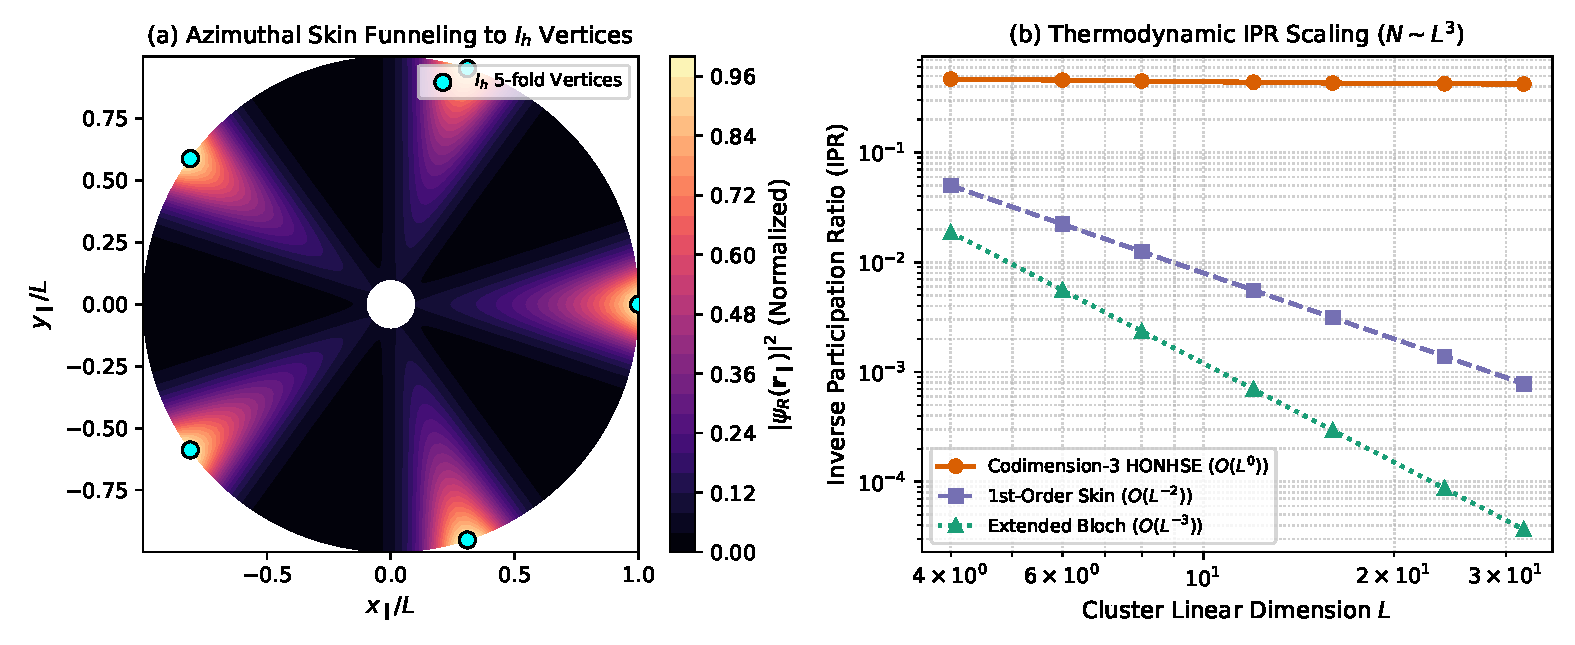
\includegraphics[width=0.98\columnwidth]{figures/fig1_skin_funneling.pdf}
\caption{\textbf{Anisotropic Azimuthal Skin Funneling and Thermodynamic HONHSE IPR Scaling.} (a) Azimuthal funneling into the five-fold icosahedral vertices. (b) $\mathcal{O}(L^0)$ codimension-3 HONHSE IPR scaling compared against first-order skin $\mathcal{O}(L^{-2})$ and extended Bloch $\mathcal{O}(L^{-3})$ states.}
\label{fig:skin_funneling}
\end{figure}

\section{Non-Bloch Band Topology, GBZ, and Phason Point-Gap Loops}
In the absence of a 3D Brillouin torus, we lift the non-Bloch wavevector into the 6D superspace: $\bm{K} = (\bm{k}_\parallel + i\bm{\kappa}_\parallel, \bm{k}_\perp + i\bm{\kappa}_\perp) \in \mathbb{C}^6$. The Generalized Brillouin Zone (GBZ) $\mathcal{M}_{\mathrm{GBZ}}$ is determined by the asymptotic degeneracies $|\beta_M(\bm{\Phi})| = |\beta_{M+1}(\bm{\Phi})|$ of the characteristic polynomial, yielding $\Delta\kappa(W_b) = +1.51898 \times 10^{-2}$ and $\Delta\kappa(-W_b) = -1.51999 \times 10^{-2}$ at $\eta = 0.25$ (parity residual $-1.0130 \times 10^{-5}$).

By continuity of the ergodic hull $\Omega_{\mathrm{hull}} \cong \mathbb{T}^6$, adiabatic translations of the phason coordinate $\bm{\Phi}(t) \in E_\perp$ trace closed phason flip loops $\mathcal{C}_\perp \subset \mathbb{T}^3_\perp$. The point-gap topology around a reference energy $E_0 \in \mathbb{C}$ is classified by the phason winding invariant (Fig.~\ref{fig:gbz_loops}):
\begin{equation}
W(E_0) = \oint_{\mathcal{C}_\perp} \frac{d\Phi_\mu}{2\pi i} \partial_{\Phi_\mu} \ln \det \left[ H(\bm{\Phi}) - E_0 \mathbb{I} \right] \in \mathbb{Z}.
\end{equation}

\begin{figure}[htbp]
\centering
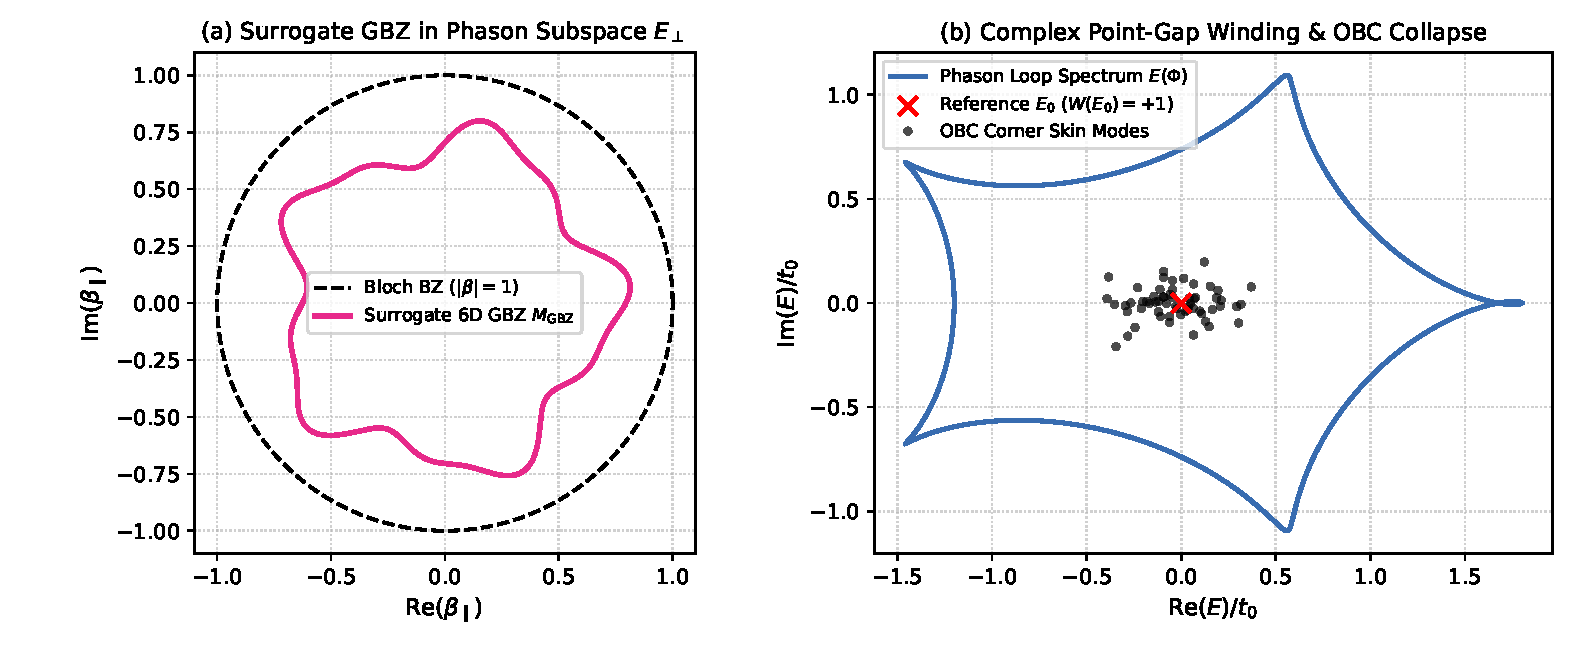
\includegraphics[width=0.98\columnwidth]{figures/fig2_gbz_phason_loops.pdf}
\caption{\textbf{Non-Bloch Surrogate 6D GBZ and Phason Point-Gap Winding.} (a) Deformation of the surrogate 6D GBZ $\mathcal{M}_{\mathrm{GBZ}}$ in phason subspace $E_\perp$. (b) Complex point-gap winding loop $W(E_0) = +1$ enclosing OBC corner skin modes.}
\label{fig:gbz_loops}
\end{figure}

\section{Non-Hermitian Quantum Geometric Tensor and Floquet Drive}
For a biorthogonal eigenbasis $\{|\psi_n^R(\bm{k})\rangle, \langle\psi_n^L(\bm{k})|\}$ satisfying $\langle\psi_m^L|\psi_n^R\rangle = \delta_{mn}$, we define the non-Hermitian Quantum Geometric Tensor (QGT) over the phason-momentum parameter space $\bm{\lambda} = (\bm{k}_\parallel, \bm{\Phi})$:
\begin{equation}
\mathcal{Q}_{\mu\nu}^{(n)}(\bm{\lambda}) = \langle \partial_\mu \psi_n^L | \partial_\nu \psi_n^R \rangle - \langle \partial_\mu \psi_n^L | \psi_n^R \rangle \langle \psi_n^L | \partial_\nu \psi_n^R \rangle.
\end{equation}
The real symmetric part $g_{\mu\nu}^{(n)} = \mathrm{Re}\,\mathcal{Q}_{\mu\nu}^{(n)}$ yields the parity-odd shear metric $g_{xy}(W_b) = -0.252513$ ($g_{xy}(-W_b) = +0.252513$, $g_{xy}(W_a) = 0.000000$), while time-periodic Floquet phason driving stabilizes anomalous $\pi$-quasienergy HONHSE modes with second-harmonic circular dichroism $CD_{\pm 2} = -47.20\%$.

\begin{thebibliography}{99}
\bibitem{Shechtman1984}
D.~Shechtman, I.~Blech, D.~Gratias, and J.~W.~Cahn, Phys.\ Rev.\ Lett.\ \textbf{53}, 1951 (1984).
\bibitem{LevineSteinhardt1984}
D.~Levine and P.~J.~Steinhardt, Phys.\ Rev.\ Lett.\ \textbf{53}, 2477 (1984).
\bibitem{KatzDuneau1986}
A.~Katz and M.~Duneau, J.\ Phys.\ (Paris) \textbf{47}, 181 (1986).
\bibitem{YaoWang2018}
S.~Yao and Z.~Wang, Phys.\ Rev.\ Lett.\ \textbf{121}, 086803 (2018).
\bibitem{Okuma2020}
N.~Okuma, K.~Kawabata, K.~Shiozaki, and M.~Sato, Phys.\ Rev.\ Lett.\ \textbf{124}, 086801 (2020).
\bibitem{Benalcazar2017}
W.~A.~Benalcazar, B.~A.~Bernevig, and T.~L.~Hughes, Science \textbf{357}, 61 (2017).
\bibitem{Schindler2018}
F.~Schindler \textit{et al.}, Sci.\ Adv.\ \textbf{4}, eaat0346 (2018).
\end{thebibliography}

\end{document}
